\documentclass[00_complete]{subfiles}

%\documentclass[12pt]{report}
\usepackage[utf8]{inputenc}
\usepackage{amsmath,amssymb,amsthm,gensymb,parskip,graphicx,footmisc,csquotes,enumerate,datetime2}
\usepackage[]{libertinus}
\usepackage[breaklinks]{hyperref}
\hypersetup{
  pdfauthor={Moshe Krumbein},
  colorlinks=true,
  linkcolor={black},
  filecolor={black},
  citecolor={black}, %blue
  urlcolor={black}, %blue
}
\usepackage[top=30mm,bottom=30mm,left=30mm,right=30mm]{geometry}
%\setlength{\emergencystretch}{2em} % prevent overfull lines
\providecommand{\tightlist}{%
\setlength{\itemsep}{0pt}\setlength{\parskip}{0pt}}

\renewcommand\qedsymbol{$\blacksquare$}

\theoremstyle{definition}
\newtheorem*{definition}{Definition}
\newtheorem*{theorem}{Theorem}
\newtheorem*{axiom}{Axiom}
\newtheorem*{lemma}{Lemma}

\theoremstyle{remark}
\newtheorem*{note}{Note}
\newtheorem*{symbols}{Symbol}
\newtheorem{example}{Example}[section]
\newtheorem*{claim}{Claim}
\newtheorem*{conclusion}{Conclusion}
\newtheorem*{reminder}{Reminder}

\usepackage{fancyhdr}
\usepackage[italicdiff]{physics}
\MakeOuterQuote{"}

\renewcommand{\chaptermark}[1]{\markboth{#1}{}}

\pagestyle{fancy}

\setlength{\headheight}{14.5pt}
\addtolength{\topmargin}{-2.5pt}

\fancyhf{}
\rhead{Moshe Krumbein}
\lhead{\chaptermark}
\cfoot{\thepage}
\fancyhead[R]{\chaptername~\thechapter}
\fancyhead[L]{\mbox{\leftmark}}

\usepackage[Rejne]{fncychap}
\usepackage{titling}

\makeatletter
\renewcommand{\@chapapp}{\vspace*{-100pt}\huge\thetitle}
\makeatother

\makeatletter
\newcommand{\subtitle}[1]{%
  {\center\vspace*{-60pt}%
  \linespread{1.1}\Large\scshape#1%
  \par\nobreak\vspace*{35pt}}
}
\makeatother

\newcommand{\Chapter}[2]{
    \def\n{#2}
    \setcounter{chapter}{\the\numexpr\n-1}
    \chapter{#1}
    \subtitle{\theauthor~- \thedate}
}

\DeclareMathOperator{\Ima}{Im}
\DeclareMathOperator{\Id}{Id}
\DeclareMathOperator{\cis}{cis}

\newcommand{\Mod}[1]{\ (\mathrm{mod}\ #1)}
\newcommand{\st}[0]{\;\mathrm{s.t.}\;}

\title{Computer Architecture}
\author{Moshe Krumbein}
\date{Spring 2023}

\begin{document}
\Chapter{Introduction}{1}
\section{History}
The ENIAC was one of the first computers, created in 1946. It was 27 tons,
required 160KW. At the time no one could imagine how or why anyone would want or
have one in their homes.

Today, computers are much more power efficient, smaller, affordable, and powerful.
\section{What does a computer consist of?}
\begin{itemize}
    \item I/O
    \item Storage (Volatile/Non-volatile)
    \item CPU
    \item OS
    \item Device Drivers
    \item Software
\end{itemize}

This course primarily covers how a CPU core operates.
\section{Moore's Law}
Intel's co-founder Gordon Moore predicted that the number of transistors on a
chip will double every two years, which has essentially been accurate for the
last 40 years.

This translates to computing performance as well as energy efficiency.

A similar explosion in development in regards to storage capacity and size.
\section{The AAA Paradigm}
Every computer scientist should master "AAA":
\begin{itemize}
    \item Architecture
    \item Algorithms
    \item Applications
\end{itemize}
\section{Apps to Physics in Steps}
This course will cover the bridge between physics and user applications.

We will cover Instruction Set Architecture (ISA) which is CPU abstraction for
programmers, for example x84, ARM, RISC-V, and MIPS. Additionally, we'll learn
about micro-architecture and Gates/Register-Transfer Level (RTL).
\section{Semiconductors}
\subsection{Transistors History}
In 1906, the first vacuum tube was invented. IN 1947, the first point-contact
transistor was built by Bell Laboratories. In 1958, the first integrate circuit
was created by Kilby at Texas Instruments.

\subsection{Chemistry}
In the late 1800's, Mendeleev created the Periodic Table of Elements, which
organized the elements by their characteristics (and the discovery of
"periodicity" to the elements).

Today we know that the characteristics of different elements has to do with the
electron configuration of the atoms of each element.

In 1913, Bohr developed Bohr's model, which models the atom as a nucleus with
electron orbits (in shells). 

Essentially, each column represents the number of electrons in the outer-most
electron shell.

\begin{figure}[ht!]
    \begin{center}
        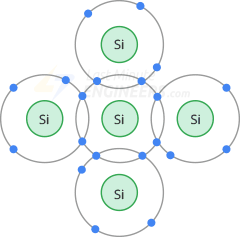
\includegraphics[width=0.5\textwidth]{silicon-crystal.png}
    \end{center}
    \caption{Silicon Crystal}
\end{figure}

Atoms "want" to have a full outer shell. A \textit{covalent bond} is where atoms
share electrons in their outer-most shells.

An \textit{ionic bond} is bonding of oppositely charged ions, where an ion is a
n atom or molecule with net electrical charge.

\subsection{Electricity}
\begin{itemize}
    \item \textit{Current} is the flow of electrons (or holes). By convention:
        from $+$ to $-$.
    \item \textit{Voltage} is electric potential, measured in Volts. 
    \item \textit{Charge} is the amount of electrons that are stored.
    \item \textit{Capacitance} is the ability to store charge.
        \item \textit{Electrical Circuit} is a loop where current flows from
            high potential to low potential. \textit{Resistance} impacts the
            rate of flow, (high resistance means it's "harder" to flow). An
            electrical circuit may include branches.
\end{itemize}
\subsection{Representing 0 and 1}
By convention, high voltage is $1$ and low is $0$. Usually a range of potential
voltages work, with an undefined in the middle.

We will use hexadecimal (base-16).
\subsection{Semiconductors}
Bad conductors in their pure form.

Common semiconductors:
\begin{itemize}
    \item Boron (B)
    \item Silicon (Si)
    \item Germanium (Ge)
    \item ...
\end{itemize}
Pure silicon is a semiconductor because it does not conduct electrical current
well, because it has few free charge carriers.
For example sand (SiO\textsubscript{2}) because it doesn't conduct any electrical current.

\textit{Doping} is the intentional introduction of impurities into an intrinsic
semiconductor for the purpose of modulating its properties. This is done by
adding atoms of a different element.

Types:
\begin{itemize}
    \item \textit{P-type semiconductor} (Silicon doped with aluminum)
    \item \textit{N-type semiconductor} (Silicon doped with potassium)
\end{itemize}
Electrical components are made using a combination of doped materials. The
combonation of N and P forms a \textit{PN junction}, which only allows flow in one
direction and not in the other. This is also known as a \textit{diode}.
\section{MOSFET}
A \textit{Metal–oxide–semiconductor field-effect transistor (MOSFET)} contains
two N type semiconductors and one P type with three terminals: \textit{source},
\textit{drain}, and \textit{gate}. It is built using to NP junctions and a
capacitor. There as the variations \textit{N-Channel} (NMOS) and
\textit{P-Channel} (PMOS).
\begin{figure}[ht!]
    \begin{center}
        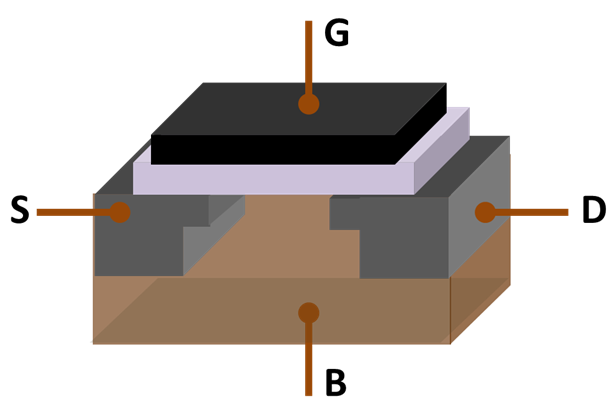
\includegraphics[width=0.5\textwidth]{mosfet}
    \end{center}
    \caption{MOSFET Structure}
\end{figure}
\subsection{NMOS Operation}
The body (P type) is always connected to ground. 

NMOS can be used as a voltage-controlled switch. It has two charged NP
junctions, current cannot flow from source to drain. This is call \textit{Gate 
"0"}. However, when there is an N-like channel between source and drain, current
can flow from source to drain. This is called a \textit{Gate "1"}.

\subsection{MOSFET Transistor}
The gate controls a 'switch-like' functionality between the source and drain.
PMOS operates in a similar way, just the opposite.
\subsection{Silicon Manufacturing}
Creating wafers. Pure silicon is melted and added to it is a small amount of
"dopant" to make it P type. Then it crystallized around an ingot and cut into
wafers.

Using light, the water is processed into 3D structures.
\section{Logic Gates}
\subsection{Inverter}
Built out of a PMOS and NMOS in parallel, such that it returns the opposite
of the input ("0" to "1" and "1" to "0").
\end{document}
